\documentclass{article}
\usepackage[utf8]{inputenc}

\title{capitoloML}
\author{Tommaso Boccali }
\date{November 2020}

% Title:
%Machine Learning for Monte Carlo simulations

%Possible TOC:

%Introduction to Neural Networks (with emphasis on generative models)
% Neural networks and Deep Learning (2 pages)
% Convolutional networks (and recurrent neural networks ?) (1 page)
% Generative models (6 pages)
%  Auto-Encoders and Variational Auto-Encoders
%  Generative Adversarial Networks
%  Graph Networks
%Example of applications for Monte Carlo simulations (of interest in medical physics and beyond) (3 pages)
% Emulation of electromagnetic interaction models (?)
% Emulation of low energy nuclear interaction models
% Emulation of radiation-matter interactions
% Emulation of detector responses (?)
% Strong and weak points about Neural Networks applications for Monte Carlo simulations (3 pages)
% Speed, accuracy and reliability
% Response to unexpected (untrained) signals
% Unphysical responses and how to impose physical constraints


%
\begin{document}
\chapter{Machine Learning for Monte Carlo simulations}
\chapterinitial{C}{omputing} techniques loosely based on mimicking the behavior of the human brain are becoming more and more important in a vast range of applications.
Their utilization is not new, with studies based on simple Neural Networks (see for example~\cite{nn1,nn2,nn3}) dating back at least to the 80s; what is instead quite recent is the possibility to deploy efficient computing architectures, often specifically tailored to the tasks

At the same time, the capability to deploy larger and larger system has triggered theoretical studies, driving to more solid bases and to  the definition of more complex and specialized models.

In these chapter we will start with an introduction to the model most relevant for Monte Carlo simulations, followed by a selection of applications. In the last part of the chapter, we will review the strong and weak points about the utilization of Neural Networks applications for Monte Carlo simulations.

\section{Introduction to Neural Networks}
Neural Networks are a specific branch of the Artificial Intelligence (AI) domain in computer science.
They get their inspiration from the fact that humans are evidently able to fulfill complex tasks; hence, by replicating the low-level mechanisms of the human brain on computing systems, one can potentially construct high level algorithms with similar capabilities.

\subsection{The human brain}
\label{subsect:brain}
Neglecting any functional description, the human brain can be described as an organ composed by neurons, glial cells, neural stem cells and blood vessels (Figure~\ref{fig:humanbrain}).
\begin{figure}[h]
    \centering
    \begin{subfigure}[b]{0.4\textwidth}
    \centering
    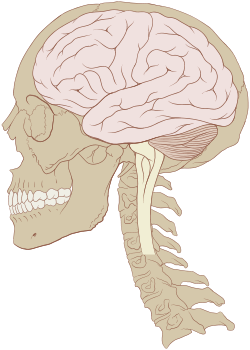
\includegraphics[width=0.6\textwidth]{images/humanbrain.png}
    \caption{A pictorial view of the human brain (from Wikipedia, by Patrick J. Lynch, CC BY 2.5).}
    \label{fig:humanbrain}
    \end{subfigure}
    \hfill
        \begin{subfigure}[b]{0.55\textwidth}
        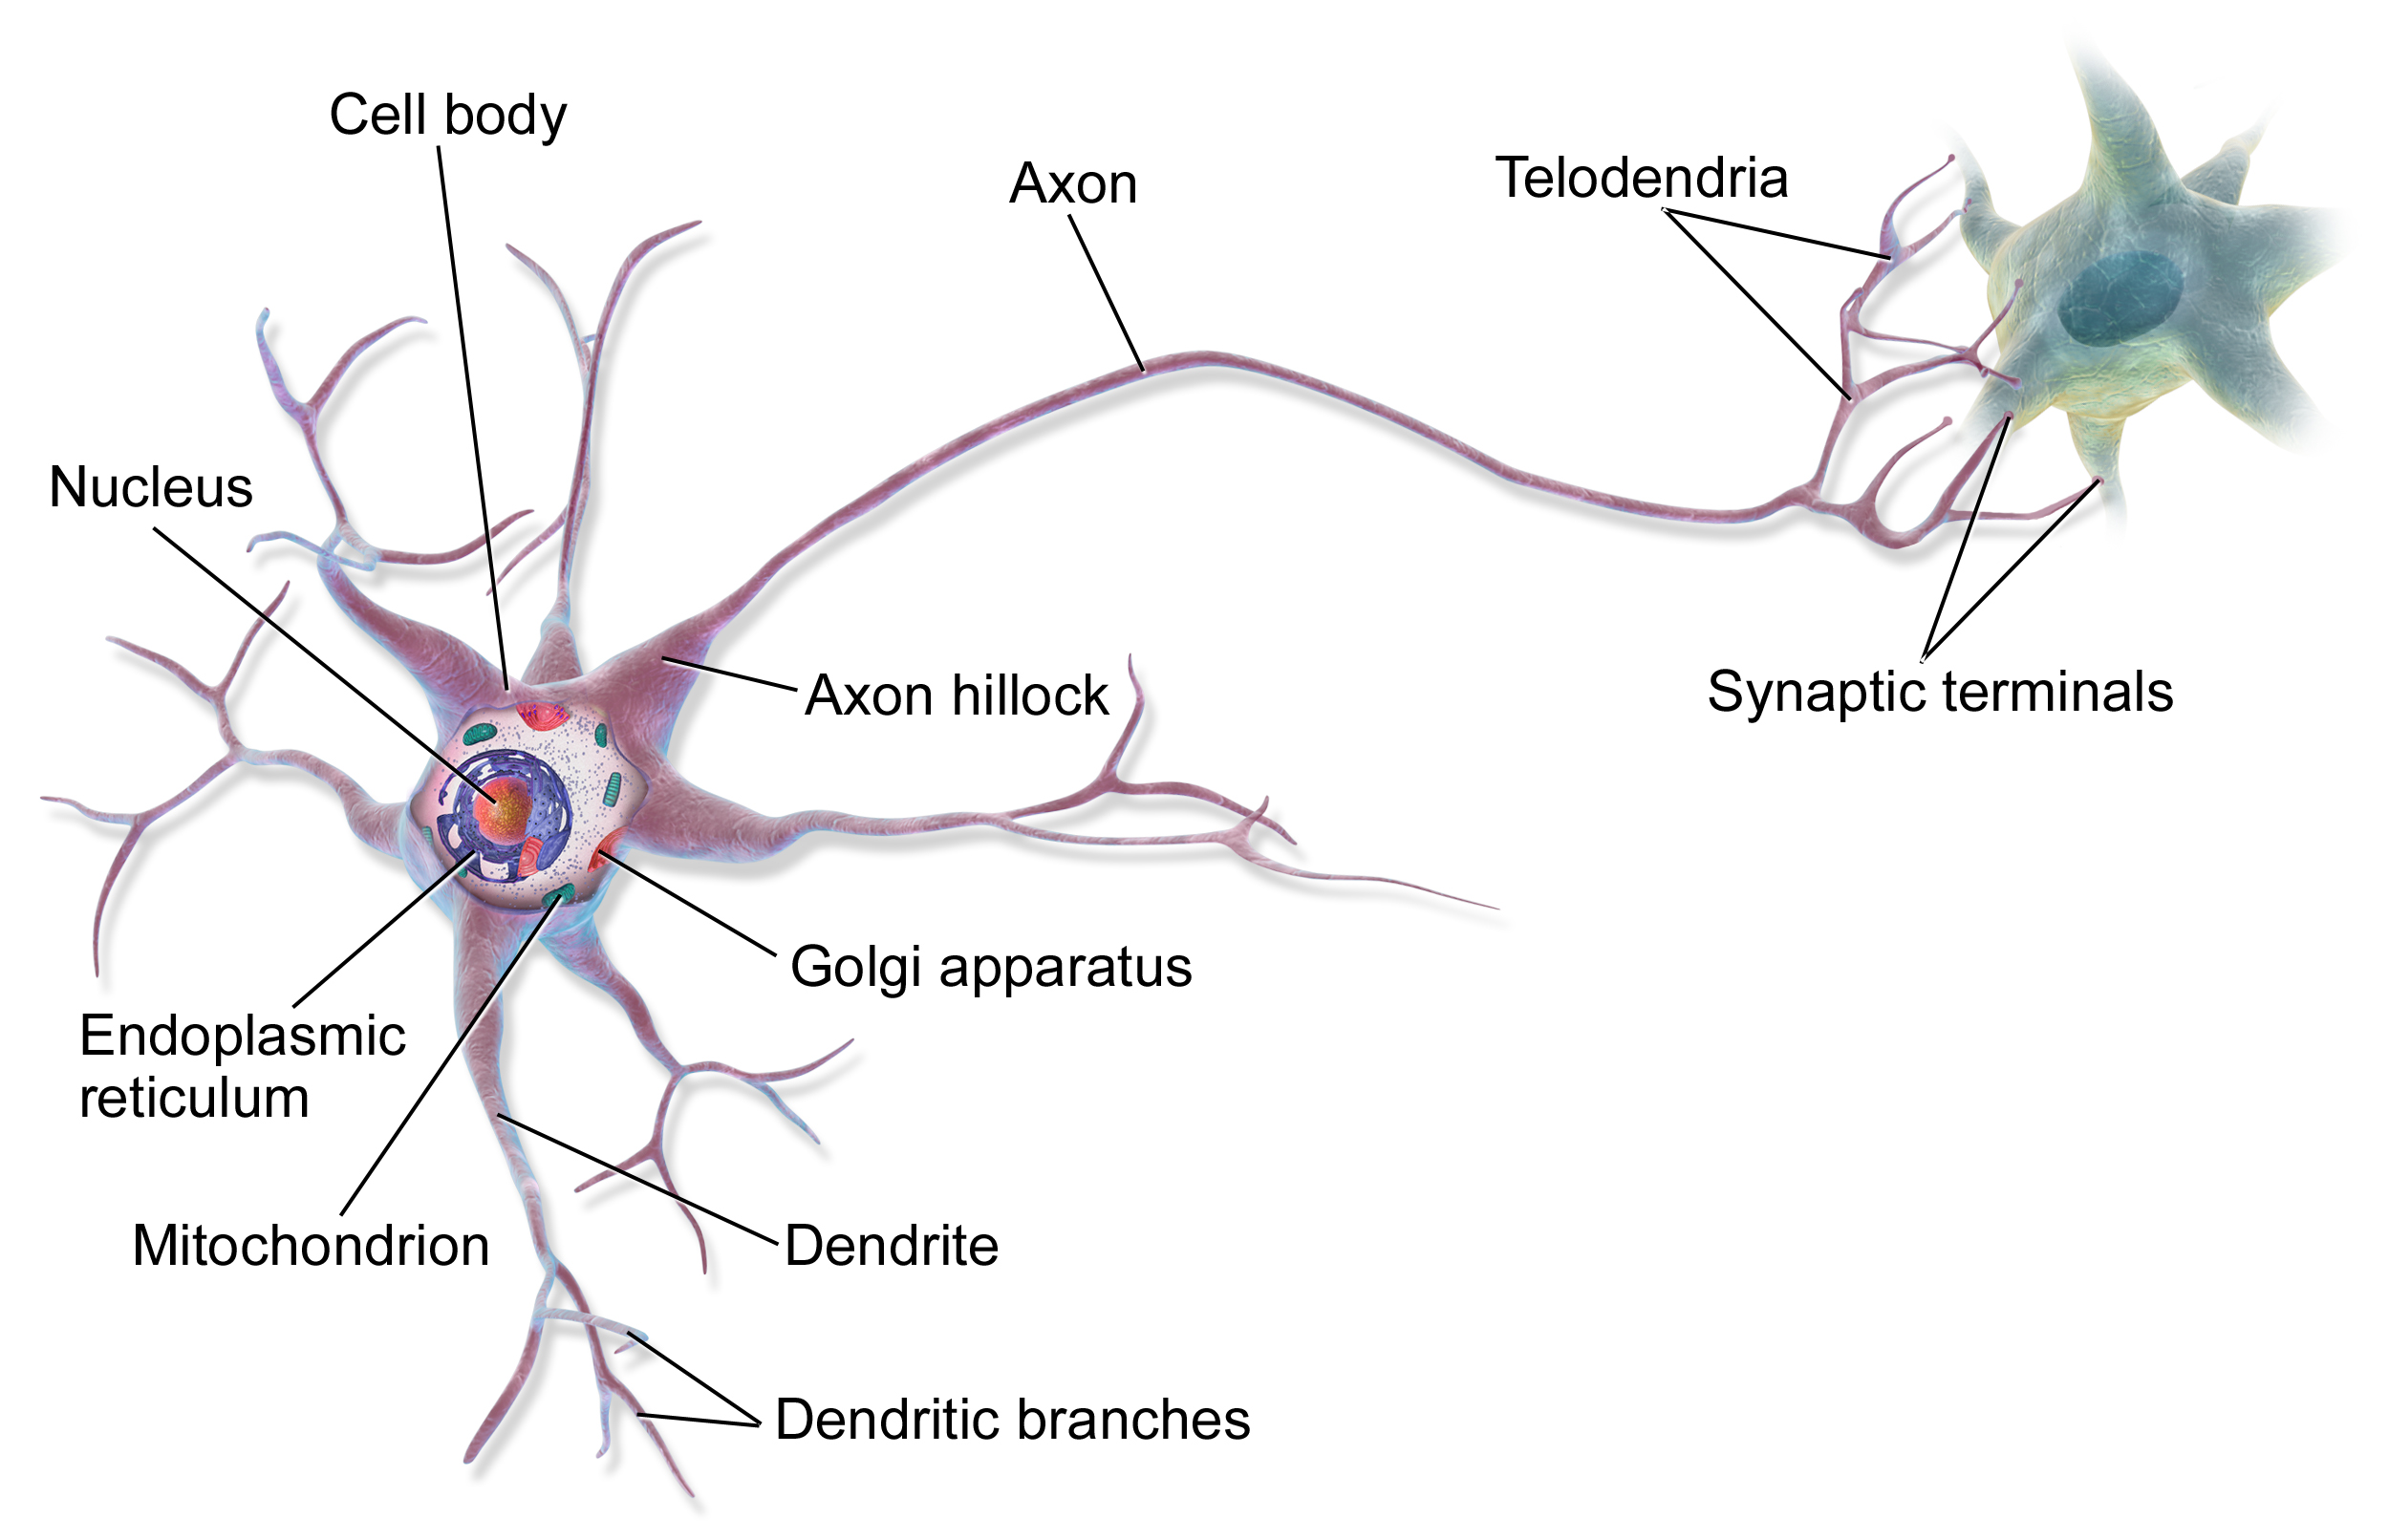
\includegraphics[width=1\textwidth]{images/Blausen_0657_MultipolarNeuron.png}
     \caption{The human neuron (from Wikipedia, by Bruce Biaus, CC BY 3.0).}
     \label{fig:neuron}
        \end{subfigure}

\end{figure}
 In our current understanding, the neurons are the units performing basic "operations" within the human brain, and their aggregated response is responsible for the high-level behaviour typical of humans.
 A neuron, as sketched in Figure~\ref{fig:neuron}, is composed of three main units: a number of dendrites, the soma (the cell body), and an axion; the total size largely varies between different types of neurons; the neurons used for cognitive functions (as those in the grey matter of the brain) are usually short, of the order of 10 mm~\cite{neuronlength}.
Functionally, a neuron is able to generate an electric response on the axion (\emph{output}), depending on the electrical potential present at the synapses (\emph{inputs}) present on the dendrites. Neurons are chained by connections between axions and dendrites, generating a mesh in which N neurons are connected via M synapses.
 The high-level response of the human brain to stimuli is understood to come from the complexity of such mesh, with a standard human brain featuring $\sim 10^{11}$ neurons each with $~7000$ synapses, for a total of $\sim 10^{15}$ ``connections''; as we will see in the following, the brain can be interpreted as a complex mathematical system with $10^{15}$ degrees of freedom.

 In literature various models of the neuron behavior have been proposed~\cite{neuronbe1, neuronbe2}; 
 here we will focus on the simplest yet most simple to implement in computer systems~\cite{artificialneuron} (see Figure~\ref{fig:artificialneuron}): %https://en.wikipedia.org/wiki/Artificial_neuron
 %
 \begin{figure}[h]
    \centering
    \hfill
        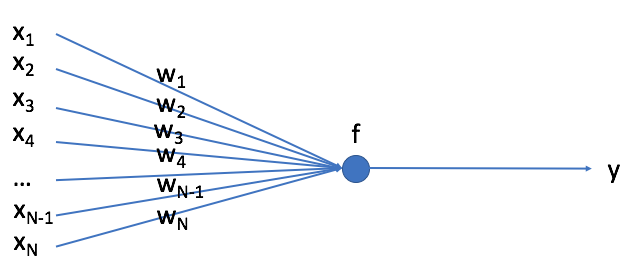
\includegraphics[width=0.9\textwidth]{images/artificialneuron.png}
     \caption{The artificial neuron.}
     \label{fig:artificialneuron}

\end{figure}
 %
 in this model, the \emph{output} $y$ signal at the axion is assumed to be a function of the \emph{inputs} $x_i$ via
 \begin{equation}
   y = f\left(\sum_{i=1}^{N} w_i x_i\right)
   \label{eq:artificialneuron}
 \end{equation}
where $w_i$ are weights modeled after the chemical potentials at the synapses, and the function $f$ wants to model the non linearity of response of biological neurons with the \emph{inputs}; on top of this, the function $f$ is needed in the mathematical model in order to allow the description of non linear phenomena~\cite{nonlinearitytheorem}. The perceptron~\cite{perceptron}, one of the first models used in literature to model Neural Networks, uses a very similar model, with a simplified $f$ function which is simply
\begin{equation}
  f(\vec{x})= \begin{cases}
                1 &  \text{if}\  \sum_{i=1}^{N} w_i x_i >0 \\
                0 &  \text{otherwise}
              \end{cases}
\end{equation}
Today, two small modifications are standard when using Neural Networks:
\begin{itemize}
\item the addition of a further synapse $x_0$ which is always 1, as a bias to the system; its weight is referred to as $x_0$ or $b$ (as in \emph{bias}).
\item the use of continuous $f$ non linear functions, as  logistic or hyperbolic~\cite{logistic} functions, in order to model non binary signals.
\end{itemize}
% logistic: https://en.wikipedia.org/wiki/Logistic_function
Neural networks are designed by combining multiple neurons in \emph{networks}, usually in a layered structure: one layer is used to map the inputs, a few/many layers are \emph{hidden}, and a single layer used to to map the outputs. On top of that, more complex neurons can be used, for example including a "memory" cell, or presenting a recurrent behavior by reusing its output as one of the inputs. A full description of all the type of neurons and networks is beyond the scope of this chapter; in the following, the ones most relevant to Monte Carlo simulations will be presented with more detail. For reference, still, a quite complete classification of currently relevant neural networks is shown in Figure~\ref{fig:types}.
\begin{figure}[h]
    \centering
    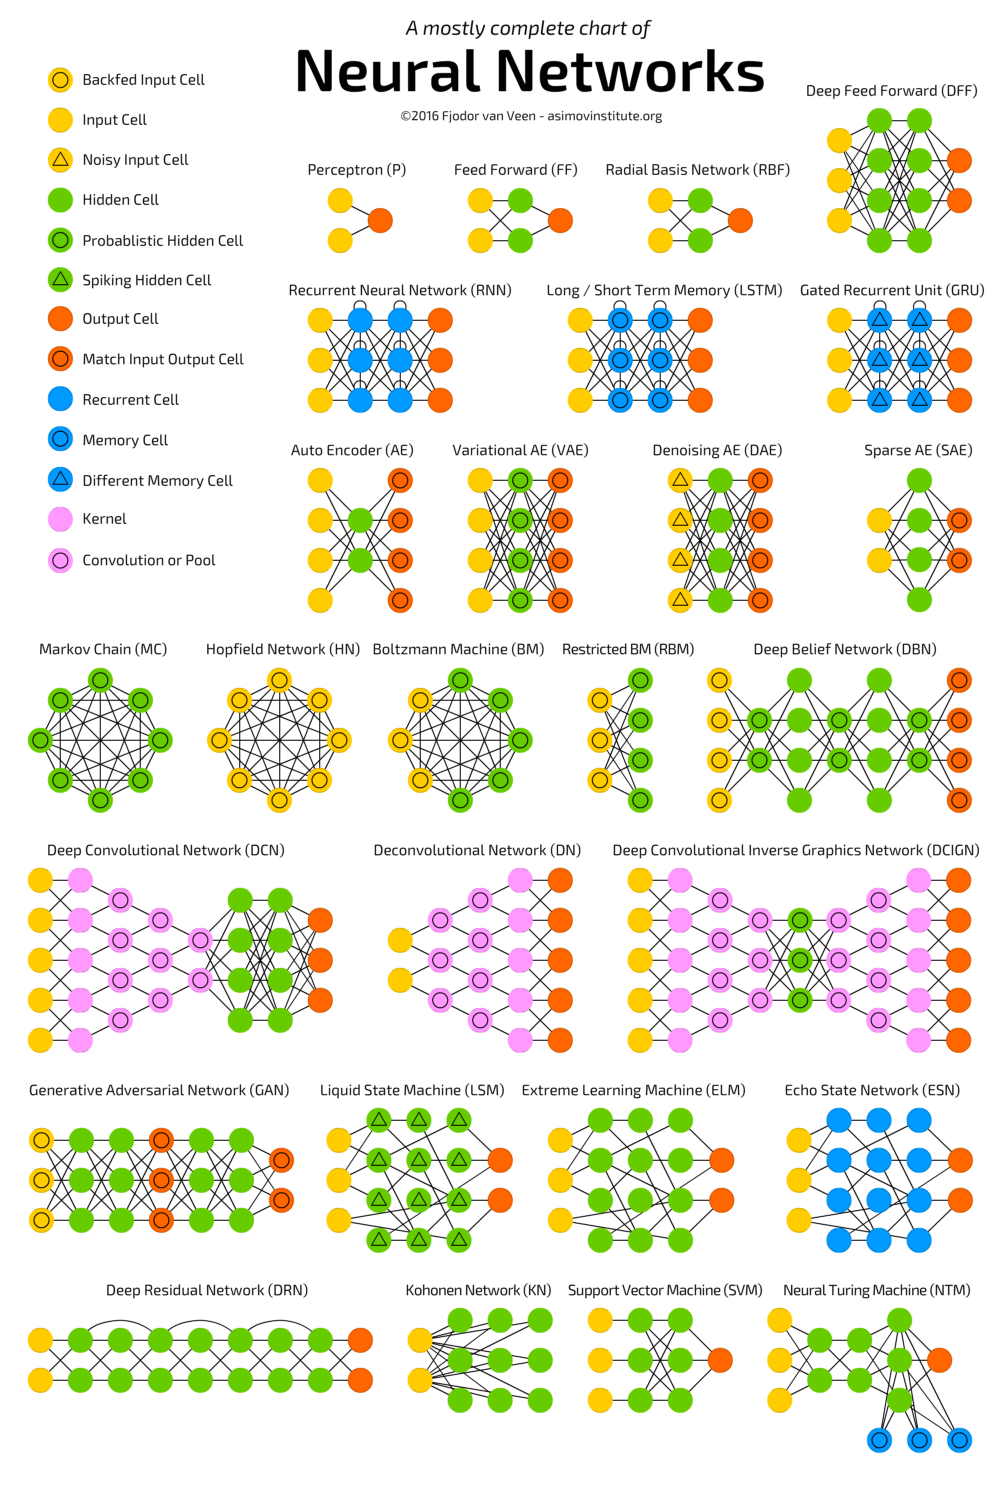
\includegraphics[width=0.9\textwidth]{images/types.png}
    \caption{Types of neurons and neural networks currently relevant in literature (Copyright F. van Veen 2016).}
    \label{fig:types}
\end{figure}

As visible in the figure, some network topologies have an high number of hidden layers. While the Universal Approximation Theorem~\cite{nonlinearitytheorem} states that, under quite generic conditions, a single hidden layer between inputs and outputs should be enough in all cases, networks used in science during the last decade tend to be ``deep'' (i.e. with many hidden layers). This has multiple motivations: on one side, the theorem states that it is possible to have just one hidden layers, but does not state with how many neurons (and it tends to be a very large number); on the other side, a deep structure tend to be better human readable, with cascade sub networks with a more identifiable and logical role. Hence, relevant networks in today's science tend to be deep.

% nonlinearitytheorem     Recommended Citation
%Kawaguchi, Kiyoshi, "A multithreaded software model for backpropagation neural network applications" (2000). ETD Collection for %University of Texas, El Paso. AAIEP05411.
%https://scholarworks.utep.edu/dissertations/AAIEP05411

The typical utilization pattern for a majority of network topologies is to feed them as input a large set of data representing the problem of interest, be it a medical image, a set of features or any output from the instrumentation, and at the same time provide the ``expected output''
from a so-called training set. 

In the simplest type of networks, the response from the neurons in the hidden and the final layers are considered in sequence (inputs to outputs), with each layer \emph{feeding} the following layers; hence the name Feed Forward Neural Networks (FFNNs).

During the training, the network adjusts its internal free degrees of freedom (the weights $w_i^j$ in equation~\ref{eq:artificialneuron}, extended to the $j$ neurons in the various layers) to better reproduce the desired answers, via minimization procedures which can be either numerical or analytical and involve the definition of a loss function to be explicitly minimized. Typical loss function can be simple weighted differences between the networks results and ``expected results'', but functional forms like cross entropy and mean square errors are more typical~\cite{lossfunctions}.

What has just been described is the training process for \emph{supervised} Neural networks, which rely on an externally provided ``truth'' to adjust for optimal performance, without having any a-priori knowledge of the physical process they want to reproduce.
Other topologies describe instead the \emph{unsupervised} Neural Networks, in which the training process just implies the utilization of datasets without the need to provide the correct answers (which can be unknown). Examples of such networks will be provided in Section~\ref{sec:unsupervised}.

\subsection{Convolutional networks}
Convolutional networks (CNNs) are a useful subset of neural networks, which exhibit peculiar characteristics of being space invariant with respect of the inputs.

They are particularly interesting in the realm of Monte Carlo simulations, since the space invariance is a valuable characteristics:  
%CM farei un esempio piu' vicino all'ambito medico
%a shower from an hadronic particle into a material, when far from the edges, 
the energy deposition of a particle into a material
does not depend on the specific entry point nor on its direction.
CNNs are used with success in categorization problems, where typical structures must be discovered into a set of input data: a typical example is the identification of lesions in medical imaging, trained on reported images by clinicians ~\cite{cnnmedical}, as depicted in Figure~\ref{fig:cnnsmedical}.

 \begin{figure}[h]
    \centering
    \hfill
        %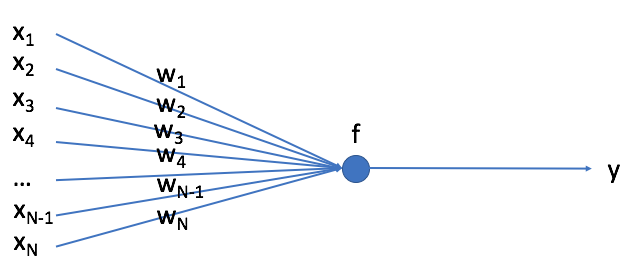
\includegraphics[width=0.9\textwidth]{images/artificialneuron.png}
     \caption{ALE SERVE UN ESEMPIO.}
     \label{fig:cnnsmedical}
\end{figure}

CNNs use basic neurons as explained in Section~\ref{subsect:brain}, with those in the hidden layers fed by small portions of the inputs per iteration, thus realizing spatial independence. Multiple application of several convolutional layers drive to an overall analysis on the inputs, and to the final outputs.

\subsection{Recurrent networks}
The CNNs above described are a type of \emph{stateless} network, in which the output depends only (given a static set of weights) on the inputs presented on the first layer. In Recurrent Neural Networks (RNNs), the response to a specific input feature set also depends on the history of the network, i.e. the inputs presented at prior times; as such, the network presents a ``memory'', which can be used to correlate multiple inputs in sequence. A typical utilization pattern is in the presence of inputs of variable length, which cannot be estimated \emph{a priori}, like in the analysis of text or speech sequences. 
In simulation processes, the feature is often utilized when the signals from a non fixed number of inputs (i.e. the incoming particles to a volume) must be piled up in a coherent way: the inputs per each particle are presented to the network, with a specific input pattern which may or may not be used to signal the end of the sequence. %A large class of RNNs can be better understood via a process called unrolling, in which the internal memomemory 

\subsection{Generative Models}
\label{subseq:gan}
The networks popular up to 10 years ago were mostly useful during a decision process, such has categorizing inputs (signal vs background, for example) or counting and defining specific regions inside it (segmentation, counting of lesions, etc).

In order to be applied to Monte Carlo simulations, instead, the capability to produce (``generate'') an output as close as possible to reality, or to a more standard algorithm is essential. In order to do this, different network topologies and strategies for training are relevant.

%It needs to be highlighted that none of the methods described in this chapter have any intrinsic knowledge of the physics involved in the simulation processes. They are "trained" on external data, which needs to be accurate as possible. While to some extent it is possible to think of a training process using data, in practice the data samples and setups to ensure a generic training is huge, and not easy to obtain in practice. Hence, standard training samples are usually provided via "old school" detailed simulation toolkits, like Geant4~\cite{g4} or FLUKA~\cite{fluka}; it is important to notice that the advent of Machine Learning techniques for Monte Carlo simulations does not imply that the latter will be less needed, on the contrary it will remain fundamental to have  understood and well tuned reference tools to be used to train AI inspired tools.

\subsubsection{Auto-Encoders and Variational Auto-Encoders}
\label{sec:unsupervised}
The autoencoders are a family of unsupervised Neural Networks designed to learn a lower dimensional representation (say N dimensions) out of a set of data (with M dimensions, M\textgreater N). The N dimension representation (``latent space'') can be seen as coming from an ``understanding'' of internal patterns and correlations in the initial data.

The easiest form of autoencoder is one in which the number of inputs and outputs equals to M, and where there is a layer at dimensionality N. The training is obtained by forcing the network during training to reproduce as close a possible the input features at the output layer, thus requesting the N-dimension space to be as perfomant as possible when representing the M-dimension inputs (see Figure~\ref{fig:autoencoder}).

\begin{figure}[htb]
     \centering
     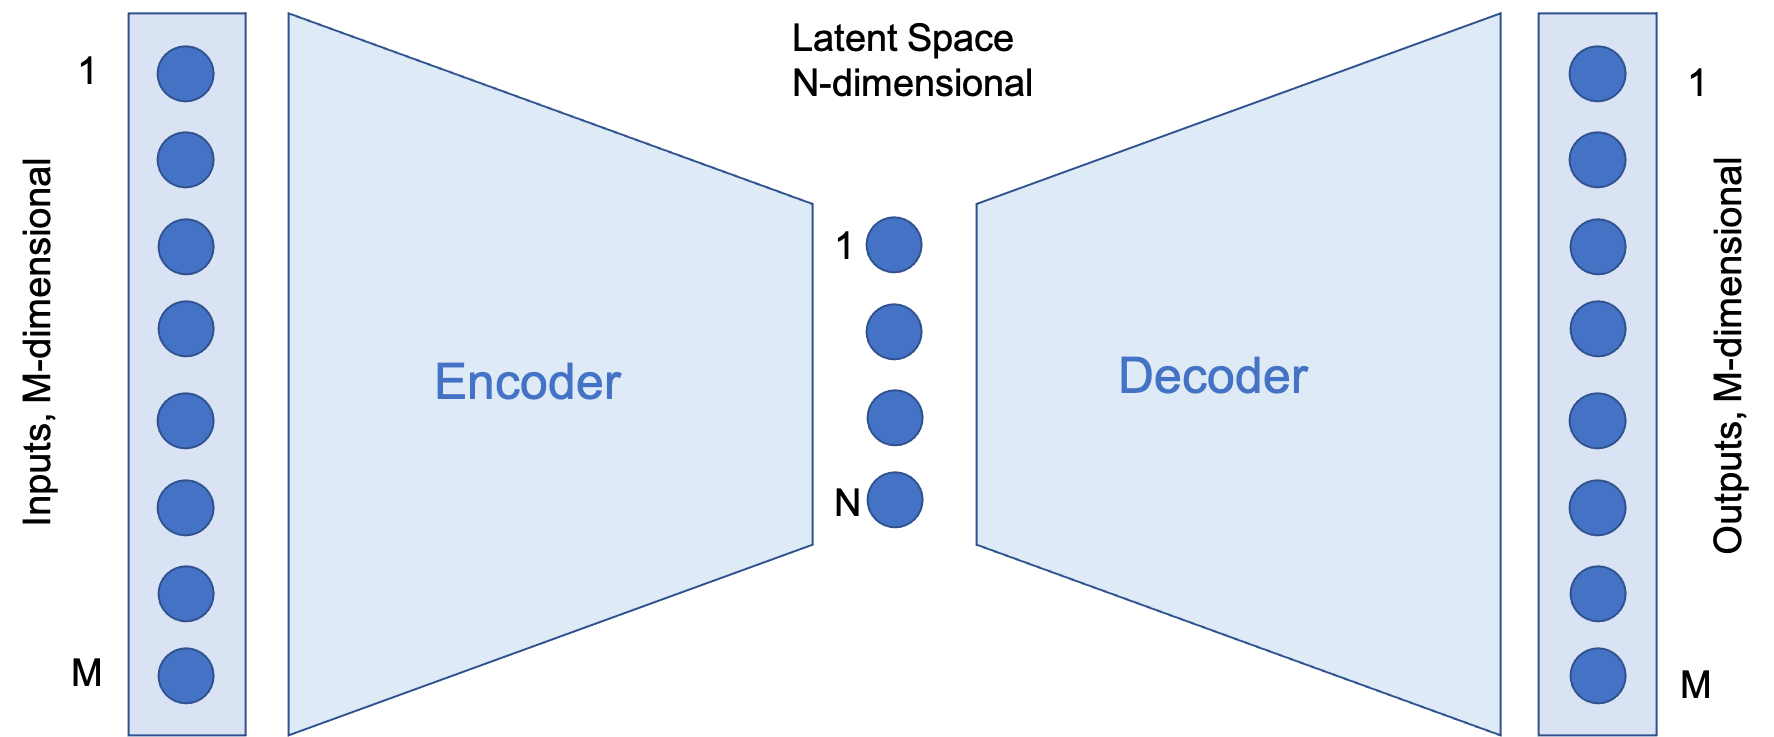
\includegraphics[width=0.95\textwidth]{images/autoencoder.png}
     \caption{An autoencoder in its simplest form.}
     \label{fig:autoencoder}
 \end{figure}
 
 Autoencoders in such form are used for two distinct purposes:
 \begin{itemize}
     \item auto-discover in the inputs hidden symmetries or underlying correlations, which can be used, for example, in lossy compression~\cite{compression} or to drive understanding on the inputs themselves; % https://arxiv.org/abs/1703.00395
     \item since the network is trained on a specific data sample, it will minimize the difference outputs vs inputs on that specific dataset. Once the same network is presented with ``different'' data, it is expected to fail to reproduce the inputs at the outputs; hence, it can be used to detect anomalous inputs, as important for the detection of not expected features, for example in medical imaging ~\cite{anomalymed} or High Energy Physics events ~\cite{anomalyhep}. 
     % https://arxiv.org/pdf/2004.03271.pdf
     % https://arxiv.org/abs/2005.01598
 \end{itemize}
 
%CM: aggiungerei piu' cose sulle VAE che sono a mio avviso la categoria di algoritmi piu' interessanti per il MC 
Auto-Encoders are only able to reproduce the elements of the training set but not to interpolate among them. Kingma and Welling \cite{vae} introduced the Variational Auto-Encoder (VAE) class of algorithms. It would be more correct to call them Auto-Encoding Variational Bayes methods 
and to introduce them with a Bayesian approach, as they are more related to Variational Bayesian methods then Auto-Encoders, however such description is beyond the scope of this book and we will give only a simplified description of them. 
The main differences of VAEs with respect to AEs is that VAEs encodes the input into a probability density function (PDF) rather than a point in the latent space, in this way close points in the latent space generate events similar to each other.
In other words, while for AEs only the points in the latent space where the the training set inputs have been encoded can be safely used to generate an output, in VAEs all the neighborhood of these points can be used.

%The naive way to generate data from a standard autoencoder 
%VAE
%It is possible to generate data from a AE, sampling random points
%is to generate random configurations 
%in the latent space of dimensionality N, and decode it with the rightmost part of Figure~\ref{fig:autoencoder} (the decoder) in order to obtain a M dimensional configuration which is ``generated'' by the network. In practice, there is no guarantee that the latent space gets organized in a way that all its points are used in the decoding/encoding process. This is where Variational Autoencoders differ: it is explicitly trained in such a way to ensure that the latent space is apt for a generative process.
VAEs, once trained to generate elements from points sampled nearby the latent space position where the training set events are encoded,
can be used to \emph{generate} realistic data, 
interpolating or extrapolating from the training set events; this make them very useful for the generation of Monte Carlo simulations.

The loss functions of AEs is a ``distance'' between the input element and the generated one; in VAEs there is another term, typically a Kullback-Leibler (KL)\cite[kl] divergence, that measures the distance between the encoding PDF and a reference PDF, usually a Normal distribution.

There is no guarantee that the latent space gets organized with respect to the input features. However, it has been shown \cite{bvae} that increasing the coefficient of the KL term in the sum of the two loss function addenda, increases the probability that the VAE learns a disentagled representation of the input. This hyper parameter is usually referred as $\beta$ and this modification of the VAE, $\beta$-VAE.

VAEs tend to produce outputs blurred with respect to inputs, however, they have the great advantage that it is possible, especially with $\beta$-VA, to control the features of the generated output and to interpolate with continuity between two input samples.

\subsubsection{Generative Adversarial Networks}
\label{subsec:gan}
Generative Adversarial Networks (GANs) are a recent~\cite{goodfellow} class of networks designed to reproduce the behaviour of complex systems without an explicit programming.

\begin{figure}[h]
     \centering
     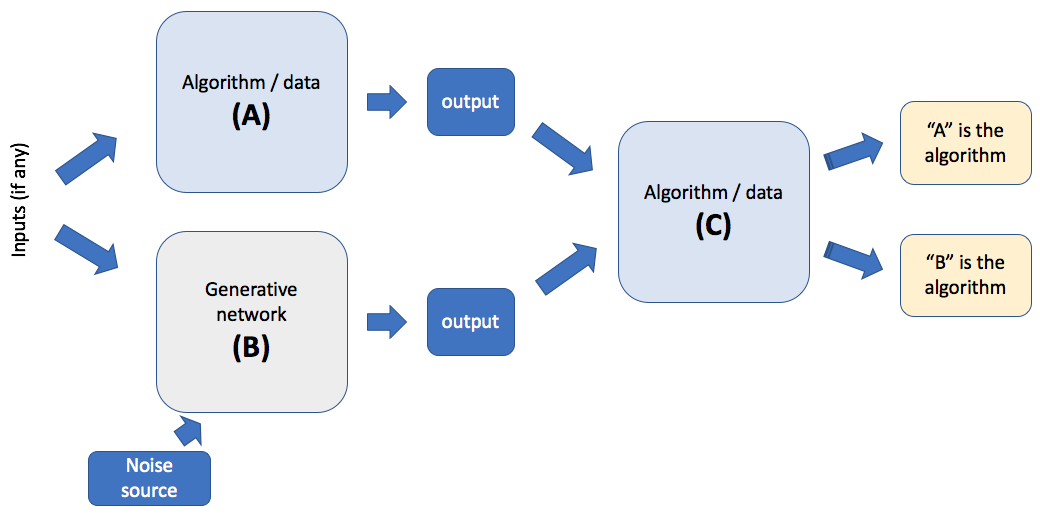
\includegraphics[width=0.95\textwidth]{images/gan.png}
     \caption{The structure of a simple GAN.}
     \label{fig:gan}
 \end{figure}

The method (see Figure~\ref{fig:gan}) implies putting in competition the reference algorithm (or real data, A) with a generative network (B), which produces an output with the same structure and whose response, initially, is random. A second network (C) is trained on the capability to distinguish between the algorithm's output and the generated one. The two networks are put in competition (hence the term \emph{adversarial}), with B "winning" if it can convince C that its response is the real one; in the opposite case, C wins.
The tension between the two networks pushes the network B to generate outputs which are indistinguishable from the real data / the output of the  algorithms. B and C are generic networks, with Convolutional neural structures mostly used.

GANs are more and more used when in the need for replicating the behaviour of a known data source, with improved computing performance. Upon successful training, in fact, the network B has the typical speed of (say) a CNN, and is able to reproduce the output of A, which can be a complex and time consuming algorithm. Successful examples are the famous generation of realistic faces~\cite{faces}, the capability to reproduce the showering of particles in calorimeters~\cite{calogan}, or for 
%the automatic segmentation of medical images~\cite{ganmed}.
for beam source modelling in Radiation Therapy linacs~\cite{Sarrut2019}.

% http://cds.cern.ch/record/2680531/files/ATL-SOFT-PROC-2019-007.pdf
% https://journals.aps.org/prd/pdf/10.1103/PhysRevD.97.014021
% https://arxiv.org/pdf/1807.01954.pdf
% https://thispersondoesnotexist.com/
% https://aapm.onlinelibrary.wiley.com/doi/10.1002/mp.13458

\subsubsection{Graph Networks}
In a quite general category of problems, the task is to discover the relations between objects; in the  segmentation of medical images, for example, there is the need to understand whether certain areas are part of a specific organs. Clusterization algorithms in many science realms is another example~\cite{clusterization}.
The most used  network architecture for these use cases is a Graph Neural Network (GNN, \cite{gnn}).
% http://citeseerx.ist.psu.edu/viewdoc/download?doi=10.1.1.1015.7227&rep=rep1&type=pdf
In a GNN, nodes (representing objects) and edges (representing connections between nodes) are the basic entities, and the training process aims to correctly categorize the nodes, via an assessment of the strength of each connection.
GNNs are finding large applications in cases where one wants to replace a complex, combinatorial algorithms with a Neural Network: typical examples in literature are jet clustering in High Energy Physics~\cite{graphclustering}, and tracking in dense particle environments~\cite{graphtracking}.
% https://arxiv.org/abs/2008.06064
% https://arxiv.org/pdf/2003.11603.pdf


% 


\section{Examples of applications for Monte Carlo simulations}
\label{sec:examples}
%guardare:

%~\cite{Sarrut2018} Sarrut D, Krah N, Badel JN, Létang JM. Learning SPECT detector angular response function with neural network for accelerating Monte-Carlo simulations. Phys Med Biol 2018;63. https://doi.org/10.1088/1361-6560/aae331.

%~\cite{Sarrut2019}
%Sarrut D, Krah N, Létang JM. Generative adversarial networks (GAN) for compact beam source modelling in Monte Carlo simulations. Phys Med Biol 2019;64:215004. https://doi.org/10.1088/1361-6560/ab3fc1.

%~\cite{Sadeghnejad-Barkousaraie2020}
%Sadeghnejad-Barkousaraie A, Bohara G, Jiang S, Nguyen D. A reinforcement learning application of guided Monte Carlo Tree Search algorithm for beam orientation selection in radiation therapy. ArXiv 2020. https://doi.org/10.1088/2632-2153/abe528.

%~\cite{Liu2020a} 
%Liu CC, Huang HM. A deep learning approach for converting prompt gamma images to proton dose distributions: A Monte Carlo simulation study. Phys Medica 2020;69:110–9. https://doi.org/10.1016/j.ejmp.2019.12.006.

%~\cite{Peng2019}
%Peng Z, Shan H, Liu T, Pei X, Zhou J, Wang G, et al. Deep learning for accelerating Monte Carlo radiation transport simulation in intensity-modulated radiation therapy. ArXiv 2019:1–8.

%\cite{Ma2020c}
%Ma S, Hu Z, Ye K, Zhang X, Wang Y, Peng H. Feasibility study of patient-specific dose verification in proton therapy utilizing positron emission tomography (PET) and generative adversarial network (GAN). Med Phys 2020;47:5194–208. https://doi.org/10.1002/mp.14443.



%\subsection{Emulation of electromagnetic interaction models}

\subsection{Emulation of radiation-matter interactions}
\label{subsec:interactions}
%tommaso
% computational cost of full fledged simulations; their not complete ability to match data
One of the most complex tasks in Monte Carlo simulations involving the use of detectors (medical apparatuses, particle physics detectors) lies in the dual need of being able to optimize the design before detector construction, and to simulate the behavior under working conditions after the setup has been prepared.
In both cases, unless the setup is very similar to existing detectors, extensive Monte Carlo simulations of the expected detector capabilities are the widely used solutions. Various such tools exist (Geant4~\cite{Agostinelli2003}, Fluka~\cite{Bohlen2014}, MCNPX~\cite{Hughes2001}), with different application regimes and specific utilization patterns. As a general rule, these implement iteratively basic radiation-matter low-level processes to a knowledge of the detector setup, including materials, geometry and  other experimental conditions; as such, they incur into two general limits:
\begin{itemize}
\item a scarce capability to be tuned to experimental results, by changing the basic modelling of the processes;
\item a large to very large need for computational resources, given the iteration oriented approach and the need to increase the level of iterations in order to obtain a better precision and adherence to data.
\end{itemize}

% Geant4, Fluka, MCNPX: https://doi.org/10.1063/1.2720459

Both limitations can in principle be surpassed via the use of Artificial Intelligence oriented tools.
In presence of experimental data, the response of the AI system can be tuned to that without any explicit modelling of the physics processes; speed can be vastly improved by the change from iteration-based computations to standard Deep Learning matrix algebra, with its intrinsic capabilities for high performance processing on, for example, GPU systems.

As an example, we want to consider here CaloGan~\cite{Paganini2018}, an attempt to reproduce the details of radiation-matter interactions in the complex setup of segmented (3 layers) electromagnetic calorimeters.
A Generative Adversarial Network, as those presented in Section~\ref{subsec:gan}, is used in conjunction with an as-accurate-as-possible Geant4 simulation of the same experimental setup. The generator side accepts in input particles' 4-momenta, and, after the passage through quite standard convolutional (matching the detector response as 2-D images) and dense layers, the output is compared with detailed Geant4 simulations of particles with the same parameters.  The training optimizes the energy deposition per layer and per 2-D transverse cell, in a way in principle suited also for using real data in input. Results are very encouraging, even in an extreme detector scenario: not only the quantities of direct training are well reproduced, but also secondary and derived quantities like shower shapes are in most cases well described.

Results are shown in Figure~\ref{fig:calogan} for the explicit targets of the calculation (2-D layered images of the energy deposits, in the specific case of incoming positrons).


\begin{figure}[h]
    \centering
    \begin{subfigure}[b]{0.55\textwidth}
    \centering
    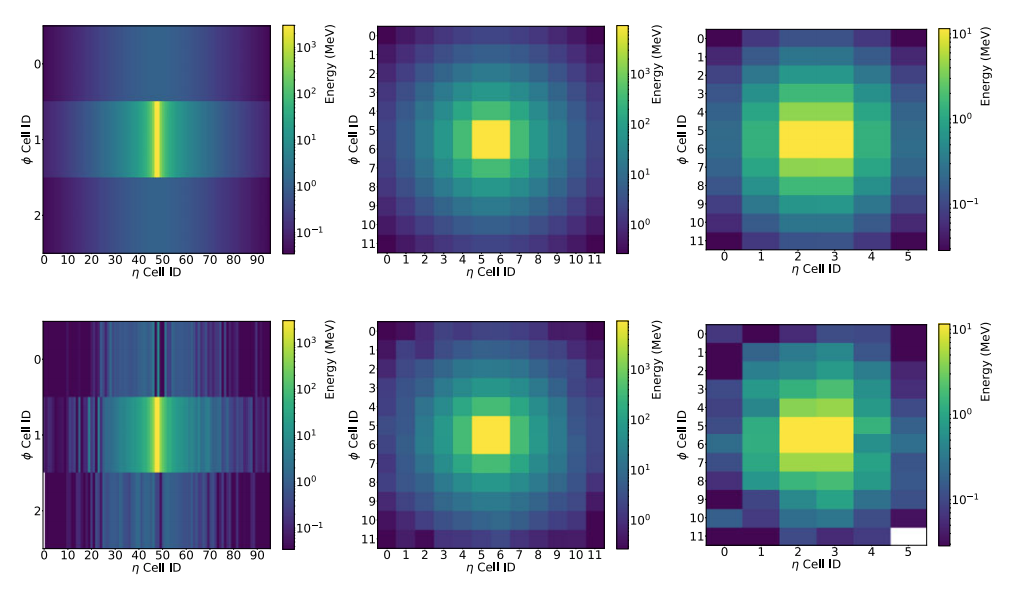
\includegraphics[width=1\textwidth]{images/calogan1.png}
    \end{subfigure}
    \hfill
        \begin{subfigure}[b]{0.44\textwidth}
        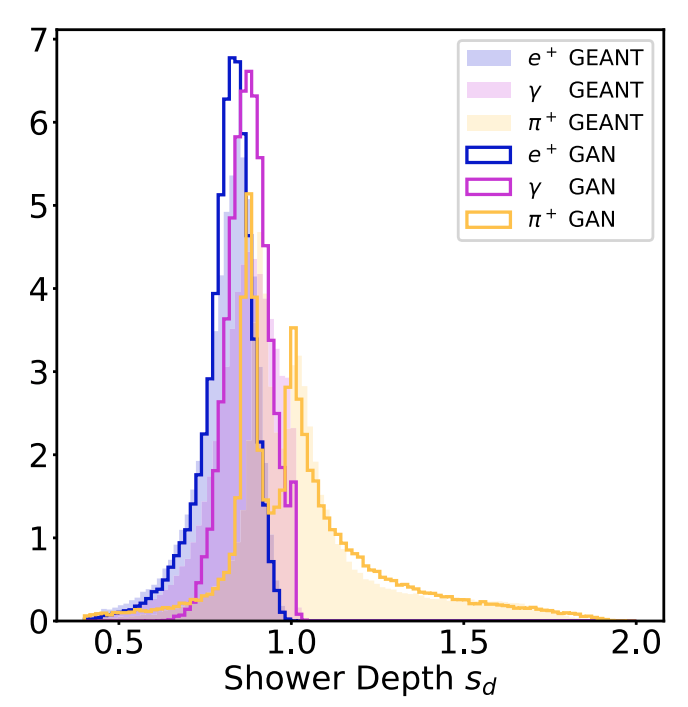
\includegraphics[width=1\textwidth]{images/calogan2.png}
        \end{subfigure}
\caption{(left) Average e$^+$ Geant4 shower (top), and average e$^+$
CALOGAN shower (bottom), with progressive calorimeter depth
(left to right). (right) Energy weighted shower depth (in a.u.) from CaloGan and Geant4 detailed simulations. (From~\cite{Paganini2018}).}
        \label{fig:calogan}
\end{figure}


Interestingly, one can look into quantities derived from shower shapes, but not directly targeted by the GAN training step, like for example the energy weighted shower depth. As we will see in Section~\ref{subsec:speed}, in general one cannot assume these quantities will be perfectly reproduced; in this specific case, though, the agreement level is quite impressive.


A second similar attempt, applied to the not-yet existing CLIC proposed electromagnetic and hadronic calorimeter, is presented in~\cite{Carminati2018}, with the goal to directly reproduce 3-D signals in a highly granular calorimeter. The reference dataset, in absence of real data, has the form of Geant4 generated showers sampled in a 25x25x25 cells around the impinging particle.
% https://doi.org/10.1051/epjconf/201921402010
Figure~\ref{fig:3dgan}(left) shows the longitudinal shower shapes for 100 GeV electrons in the electromagnetic part of the calorimeter compared with detailed Geant4 simulations. The level of agreement is very satisfactory. Figure~\ref{fig:3dgan}(right) shows a pictorial rendering of the expected energy deposit by a 100 GeV electron in the calorimeter.



\begin{figure}[h]
    \centering
    \begin{subfigure}[b]{0.54\textwidth}
    \centering
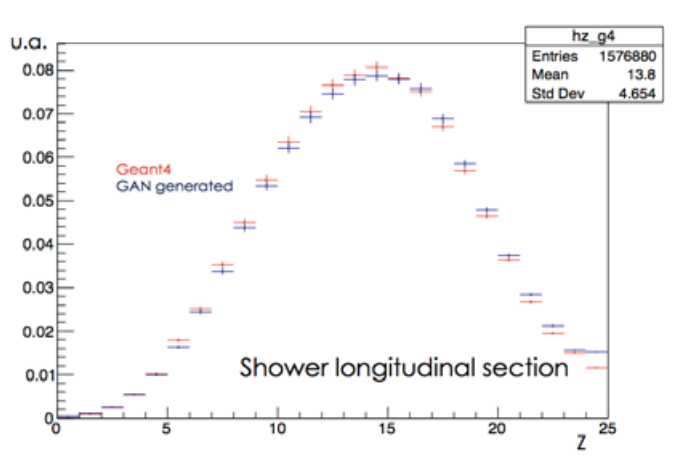
\includegraphics [width=\textwidth]{images/3dgan.png}
    \end{subfigure}
    \hfill
        \begin{subfigure}[b]{0.44\textwidth}
        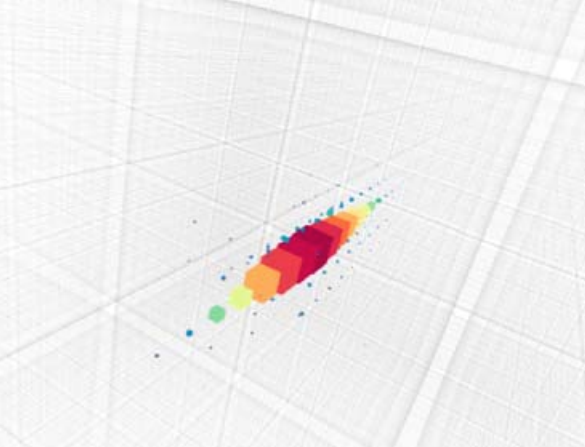
\includegraphics [width=\textwidth]{images/3dgan1.png}

        \end{subfigure}
        \caption{(left) Longitudinal shower shapes for 100 GeV electrons: GAN result is compared to full Geant4
simulation. The Z coordinate indicates the bin index in the longitudinal direction. (right) The three-dimensional representation of an energy shower created by a 100
GeV electron as generated by the GAN, using particle type as conditioning information. (From \cite{Carminati2018}).}
        \label{fig:3dgan}

\end{figure}

In sections~\ref{subsec:speed} and ~\ref{subsec:physical} we will discuss about the speed gain with respect to standard methods, and solutions and needs to prevent unphysical results.

%CM aggiungerei una frase sulle potenziali applicazioni mediche
The last two examples are related to High-Energy particle Physics, however, a similar approach can be used also to emulate the energy deposition in a voxel geometry, such as the CT of a patient.

In the field of hadron therapy, strong requirements are imposed on the accuracy in predicting the range of the treatment field in patients, and the development of patient specific dose verification methods is highly desired. Positron Emission Tomography (PET) imaging can be used to monitor the activity generated in the body tissues by the interaction with the therapeutic hadronic beams. Attempt to establish the correlation between the activity measured with a PET detector and the dose released to tissues have been carried out by utilizing  machine learning techniques based on RNN in the study by Hu et al.~\cite{Hu2020} and on GAN in the study by Ma et al.~\cite{Ma2020c}. Imaging the prompt gamma radiation is another approach to dose monitoring in hadron therapy. A deep learning based conversion of the prompt gamma information into proton dose distribution has been proposed by Liu et al~\cite{Liu2020a}. 


\subsubsection{Emulation of detector responses}
Monte Carlo tools like Geant4 are designed to simulate, as accurately as possible, the energy deposition (in keV, for example) due to the passage of particle / radiation in the material of a detector. In real life, what a scientist measures is instead the response, as analog or digital signals, of a measuring device in which energy deposition is read and processed by some electronic boards. In classical systems, the simulation of radiation-matter must be followed by an ad-hoc simulation of the electronic readout system, in order to be compared with actual readings from a detector. In the case of AI inspired tools, this can be avoided by completely bypassing the ``energy deposition'' output results, and training the system directly with real or realistic (from the above ad-hoc simulation) signals from the electronic back-end  (see Figure~\ref{fig:elec}).
%In~\cite{mri}, for example, images from a real MRI apparatus are used for the training the system (see Figure~\ref{fig:elec}); 
%the use of more classical approaches would be indeed more problematic since there is no practical way to measure (and validate) the output in terms of energy deposition in a running system.

MC simulations are also frequently used to estimate the efficiency and the geometrical acceptance of a detector, or a  system of detectors. The simulation of a Single Photon Emission Computed Tomography (SPECT) is usually done in two steps: the first one simulates the interactions of the produced photons with the patient, producing as output the emerging photons; and the second one simulates the response of the collimator-detector system to the emerging photons. This second step is called Angular Response Function (ARF).
Sarrut et al.~\cite{Sarrut2018} used a GAN to emulate the ARF. The DL algorithm takes as input the incidence angles of the photon and its energy and gives back the probability of detecting it in one of the possible energy windows. %CM: in realta' ho letto che l'output di una rete simile non può essere considerata una probabilita'
In summary, the DL algorithm emulates the detector system, including the collimators.

\begin{figure}[h]
    \centering

    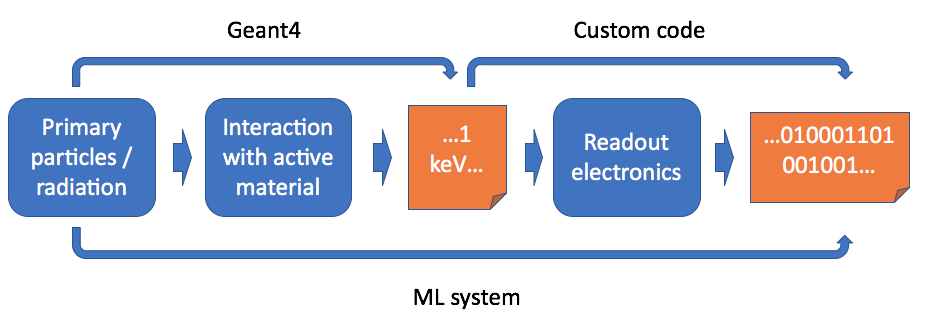
\includegraphics[width=0.8\textwidth]{images/electronics.png}
    \caption{Difference between classical and AI inspired simulation of experimental setups.}
     \label{fig:elec}

\end{figure}

%ale: trovi tu una referenza decente questo
%tommaso

\subsection{Emulation of nuclear interaction models}
Nuclear reactions models are one of the most demanding part of a MC simulation in terms of running time. Despite the large running time, the models already available in toolkits made to develop MC simulation, such as Geant4, have shown severe limitations in reproducing experimental data below 100~MeV/u~\cite{Arce2021}. Models developed by theoreticians for this energy domain can be interfaced with Geant4 with good results~\cite{Mancini-Terracciano2019}, however their running time is even larger. Ciardiello et al.~\cite{Ciardiello2020} obtained encouraging preliminary results 
in emulating one of the state-of-the-art models for low energy nuclear reactions with a VAE. The model in question is BLOB (``Boltzmann-Langevin One Body'')~\cite{Napolitani2013}, which simulates the first part of the nuclear reaction, i.e. from the contact of the two nuclei until the energy of the nucleons composing the fragments is balanced among them. The BLOB output is a PDF of finding a nucleon in a given position of the phase space. The authors trained a VAE in reproducing the BLOB prediction in the interaction of two $^{12}$C nuclei at 62~MeV/u. For this purpose, they discretized and reduced the dimensionality of the BLOB output to use 3D convolutional layers. In detail, the dimensionality reduction uses the fact that in the reaction in exam BLOB predicts at most three large fragments, i.e. larger than one nucleon. Therefore, they divided the PDF produced by BLOB in three PDFs, one per large fragment, and associated all the nucleon emitted in the first part of the reaction to one of these three large fragments. In this way they used the three colour channels of convolutional layers to represent each of the possible large fragments. In spite of controlling the generative part, they trained a classifier for the event impact parameter ($b$) jointly with the VAE itself. This joint training helps the VAE in learning a the task, given the large sparsity of the input, and forces the latent space in being organised with respect to the impact parameter. Moreover, it will be possible to sample from the latent space deciding the impact parameter of each generation.
Figure \ref{fig:out} shows that the VAE is able to generate PDFs very similar to the input one when sampling a point nearby the position in the latent space where the input has been encoded.

%\begin{figure}[!bht]
%\centering
%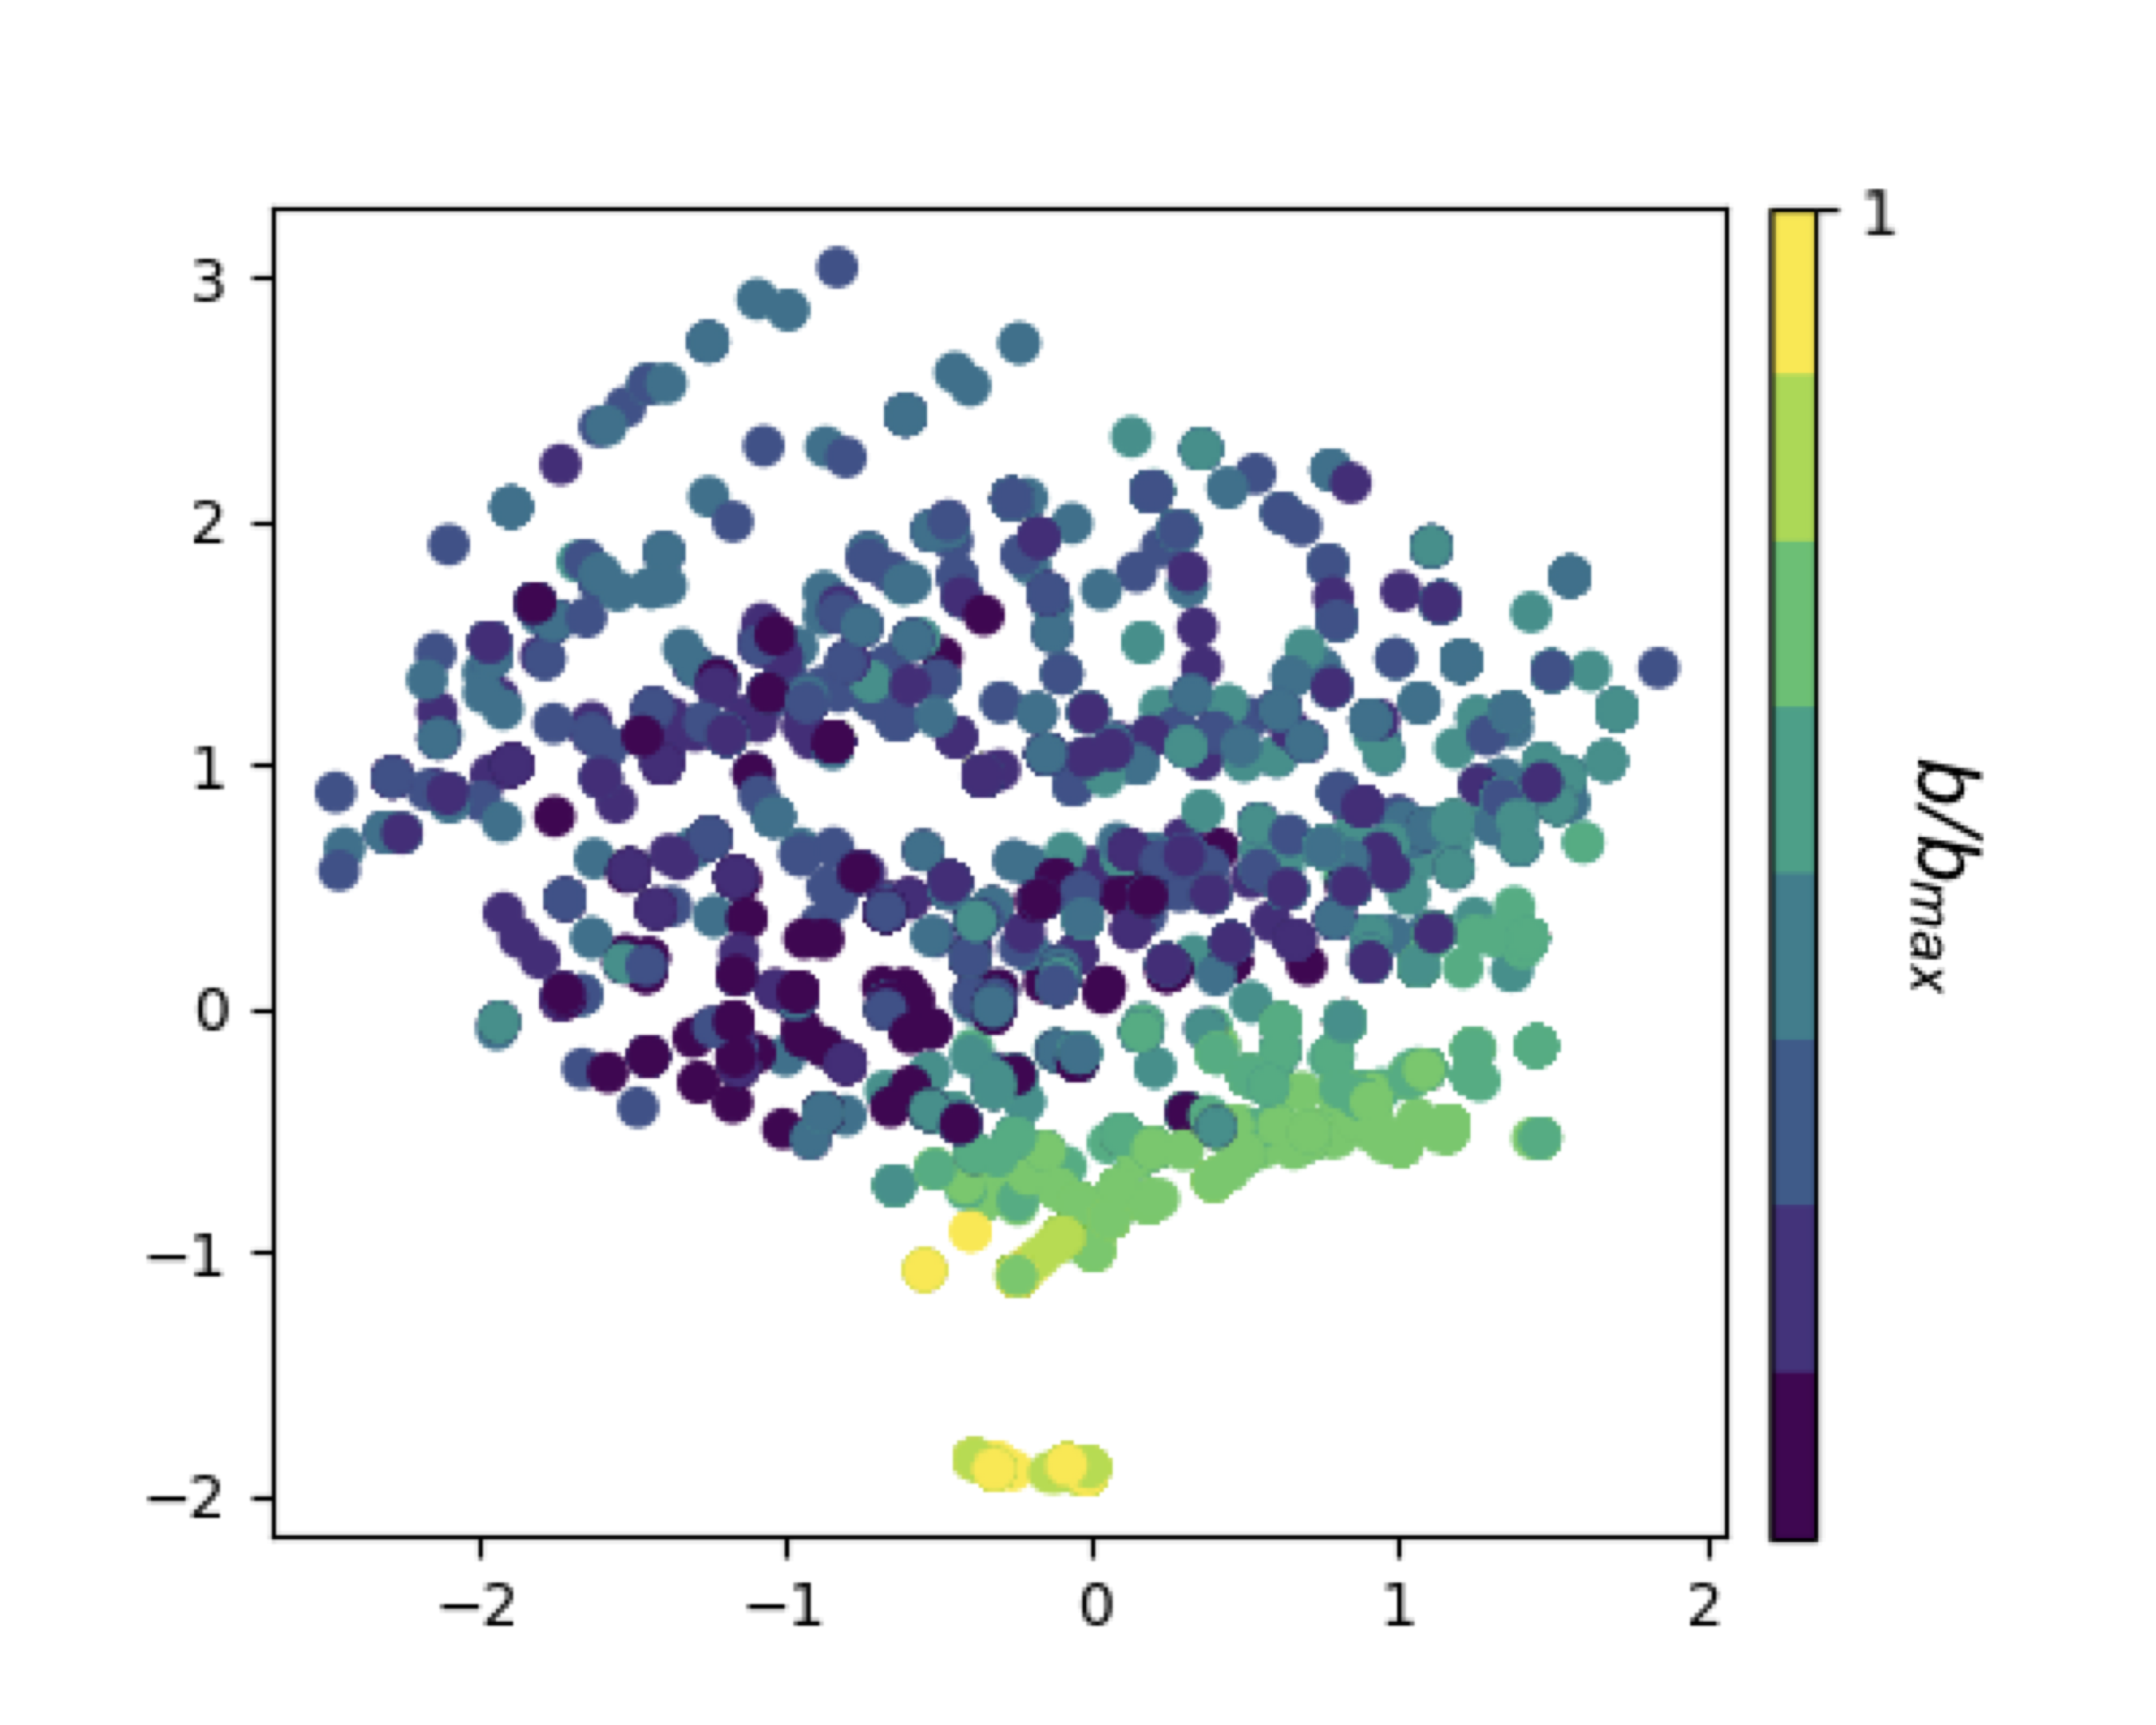
\includegraphics [width=.7\textwidth]{images/latent3}    
%\caption{Representation of the VAE latent space described in the text. Each point is the encoding point of one training %distribution, the color scale represent the impact parameter of the event.}
%\label{fig:latent}
%\end{figure}

\begin{figure}[!bht]
\centering
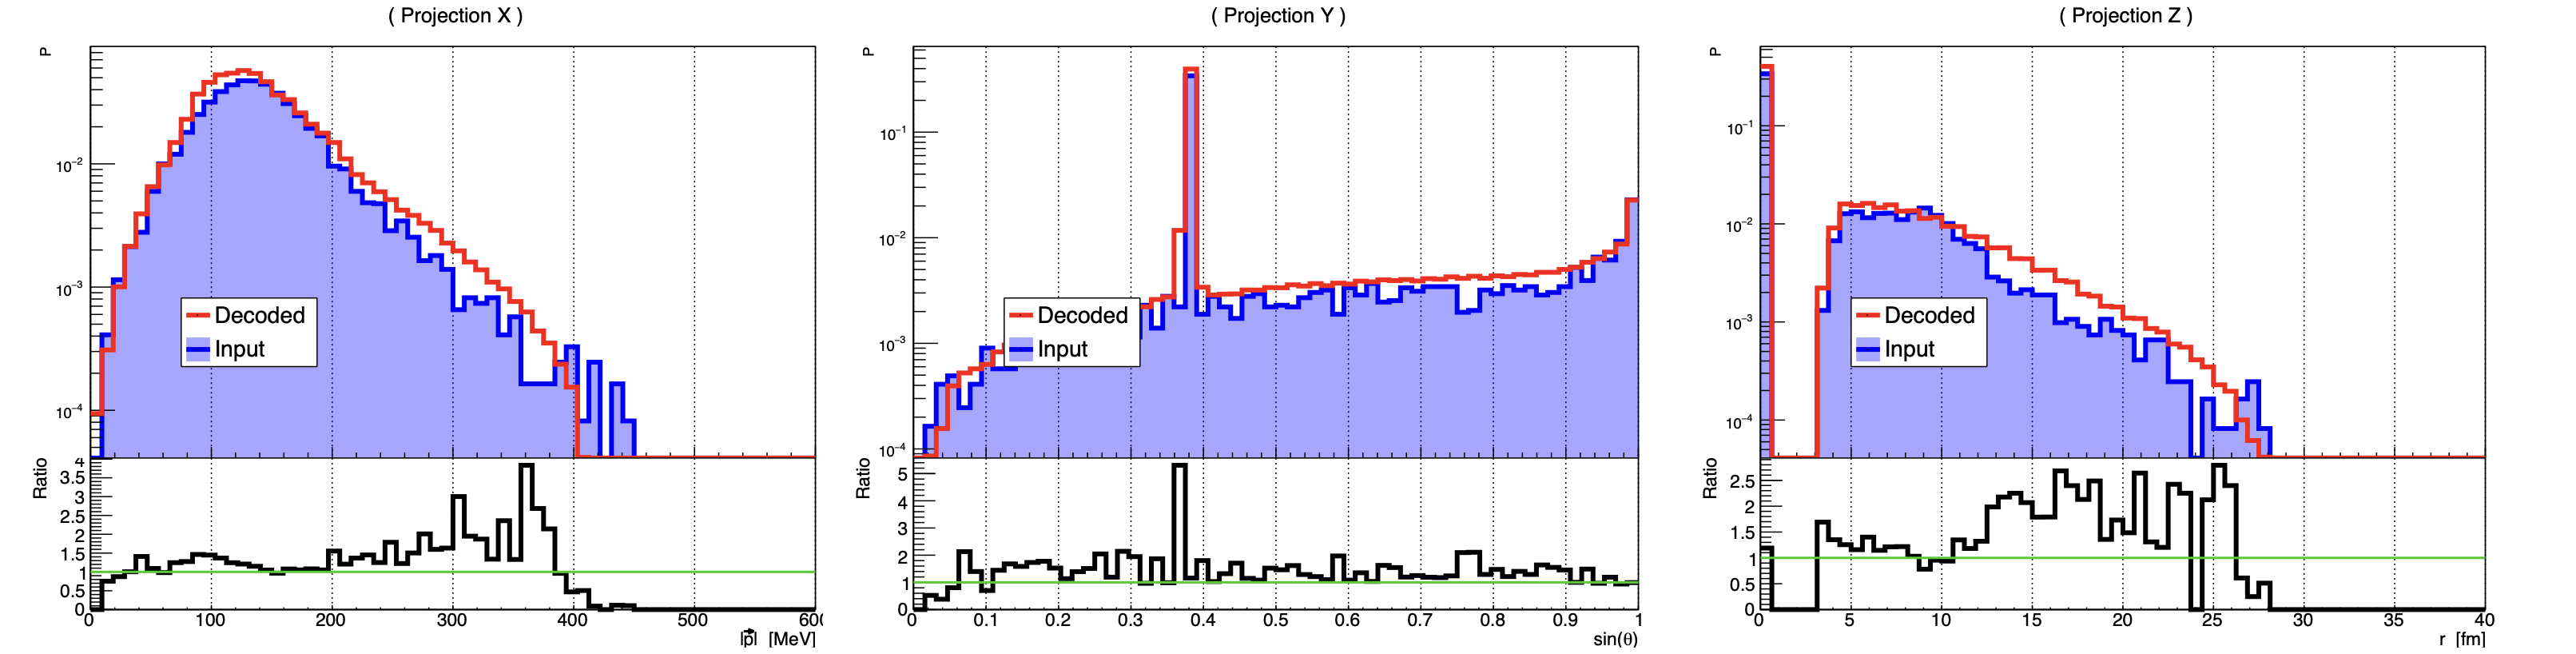
\includegraphics [width=\textwidth]{images/generated}
%\includegraphics [width=.9\columnwidth]{images/cy1}
%\includegraphics [width=.9\columnwidth]{images/cz1}
\caption{Example of results obtained in generating with the VAE a distribution, in red, starting from a point sampled from the neighborhood of the point where the input distribution, in blue, is encoded. The three distributions are the projections on the three axis of 3D PDFs. Plot from~\cite{Ciardiello2020}.}
\label{fig:out}
\end{figure}

%They conclude their work planning to enlarge the VAE latent space and train the VAE with different projectile energies and using different ions as projectile and target besides interfacing the VAE decoder with Geant4,
% so that it will be possible to use BLOB
% for simulating low energy nuclear interactions without its computational overhead

%\begin{figure}[!bht]
%\centering
%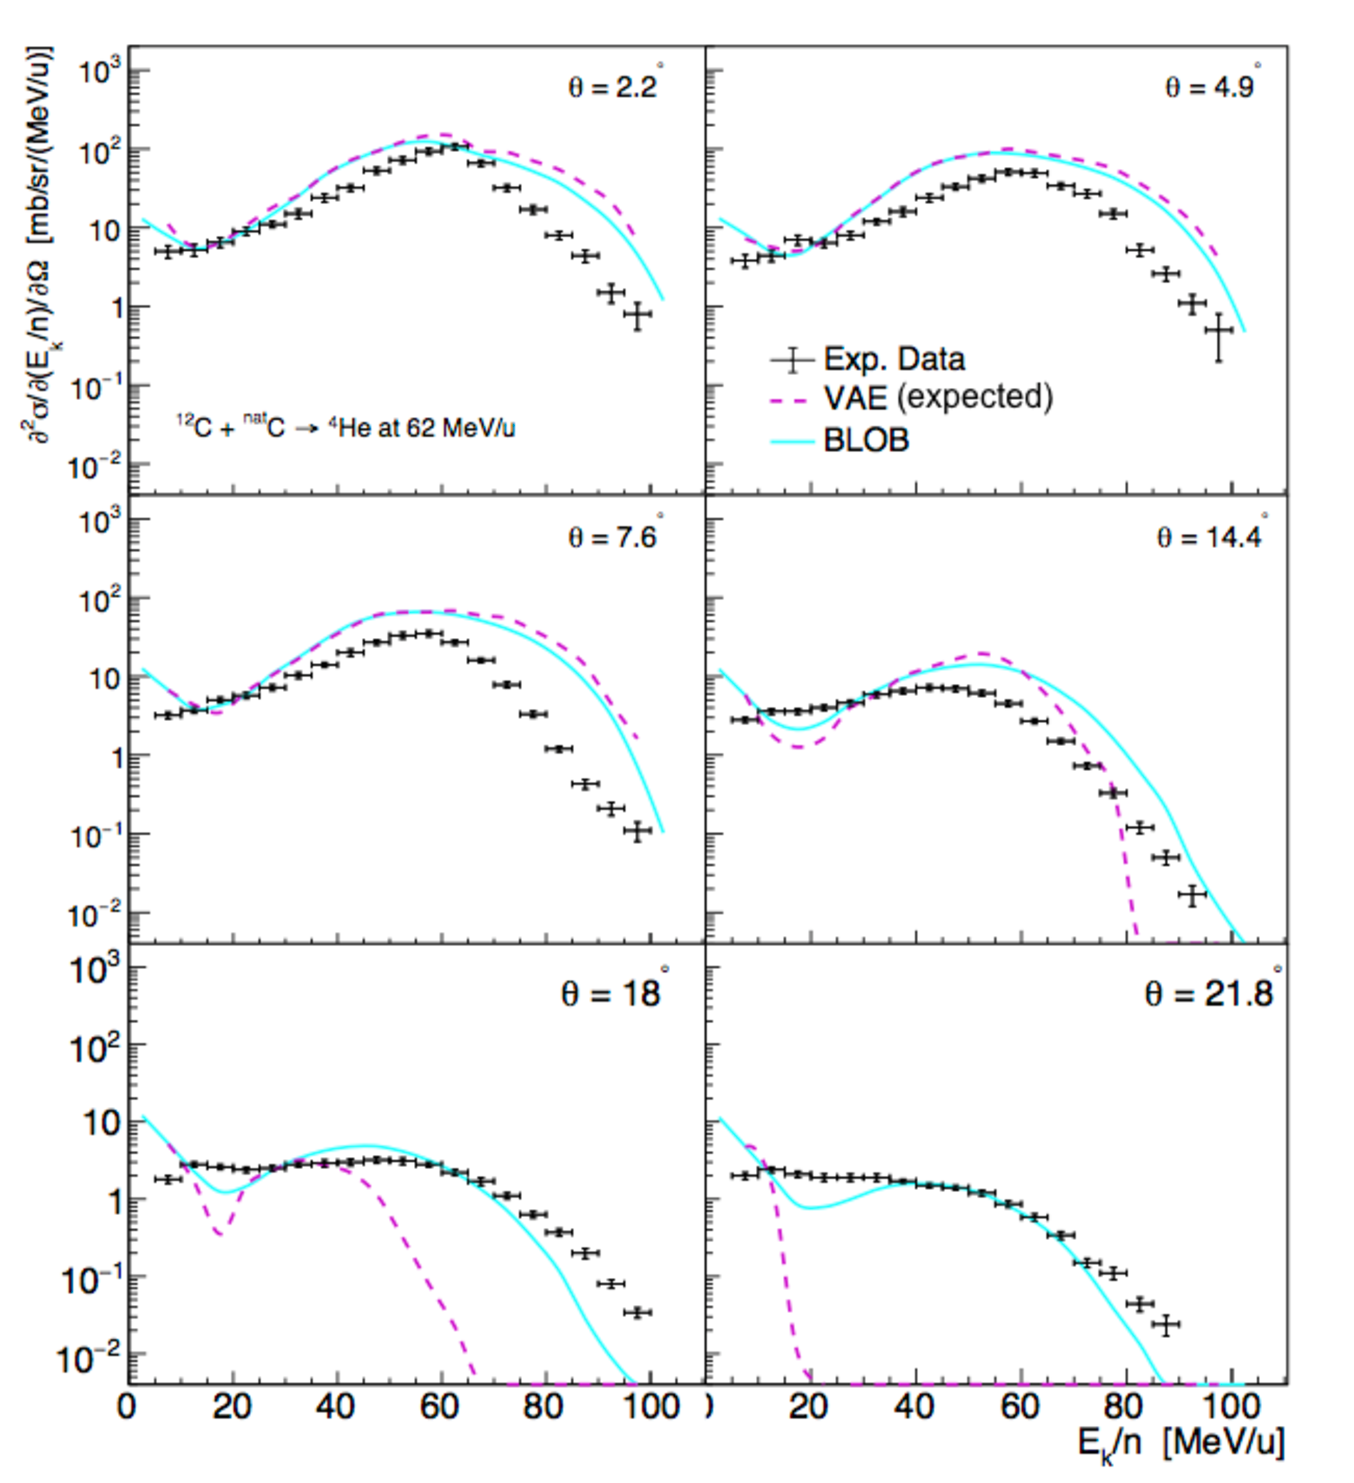
\includegraphics [width=.9\columnwidth]{images/test_reco}
%\caption{Double differential cross sections of alpha particle production in the reaction of $^{12}$C on a thin $^{12}$C target at 62~MeV/u as a function of the kinetic energy of the produced fragment for different angles. The experimental data, in black crosses, are from De Napoli et al.~\cite{DeNapoli:2012bs}. The continuous light blue lines show the BLOB predictions and the dashed magenta lines show the calculated values once encoded to reduce the PDF dimensionality and then decoded back.}
%\label{fig:testreco}
%\end{figure}

\subsection{A possible application of Graph Neural Networks}
To date, no specific study on Monte Carlo simulations of radiation / matter interactions using Graph Networks can be found in literature; still, it is clear from studies in other scientific domains suggest the potential of the technique. 
We want to cite here a study simulating the mechanical behavior of a fluid system, which shows capabilities of rendering the physics behind a complex system such as an ensemble of water small volumes~\cite{Sanchez-Gonzalez2020}; we expect similar GNN systems to become available for our research fields in short time.

\section{Strong and weak points about Neural Networks applications for Monte Carlo simulations}
Different AI based techniques for Monte Carlo simulations have been presented in literature, as shown in Section~\ref{sec:examples}; their level of maturity varies between proofs of concept, advanced tests and production systems. Still, while we may be convinced that Neural Networks can be a reasonable substitute for classical algorithms, that would not be enough in absence of clear advantages in other areas.

\subsection{Speed, accuracy and reliability}
\label{subsec:speed}
As described in Section~\ref{subsec:interactions}, one of the main expected advantage of AI inspired systems, when compared to more standard simulation algorithms, is a potential speed-up without necessarily impacting performance.
The improvement comes from the nature of feed-forwards Neural Networks used at inference time, which are described as a series of matrix multiplication of fixed length\footnote{This is not strictly valid for some types of recurrent networks, where the recurrence can introduce an indetermination in the sequence of mathematical operations.}, without access to any data structure apart from the inputs and the weights. Today's processors, from CPUs to GPUs to TPUs, are very efficient in processing matrix algebra calculations; this reflects directly to short processing times.
In order to give quantitative examples, we can refer to the two complex GANs described in Section~\ref{subsec:interactions}, which are fed by Geant4-processed events in the training phase.
Table~\ref{tab:speed} reports on the absolute time needed to process Geant4 vs the GAN for events with similar input; the speedups are of order 100x using CPUs, and an additional factor 100x with GPUs\footnote{It can be said that it is an unfair comparison since Geant4 cannot currently use GPUs; still, it shows how AI inspired tools offer a path to the use of more performing technologies.}.
\begin{center}
\begin{tabular}{l|c|c|c}
    System & Software & Speed \\
    \hline
     Intel Xeon E5-2683 & Geant4 & ~ 1 min \\
     Nvidia RTX 1080 & 3d-GAN & 0.04 msec\\
          \hline
     AWS \verb!p2.8xlarge!  & Geant4 & 1.7 sec \\
     AWS \verb!p2.8xlarge!  & CaloGan & O(10) msec \\
     AWS \verb!p2.8xlarge!  + Nvidia K80 & CaloGan & O(0.01) msec
\end{tabular}
Fig~\ref{tab:speed}: Geant4 vs GAN performance under various setups, as extracted from~\cite{Paganini2018} and~\cite{Carminati2018}.
\label{tab:speed}
\end{center}
So, speed-wise there is a clear advantage; but what about the accuracy of the simulations? 
We can refer back to Figures~\ref{fig:calogan} and \ref{fig:3dgan} to compare the reference (detailed simulations) with AI predictions. In general, a perfect agreement is not to be expected, but in many applications a O(10)\% agreement at the much reduced cost is a viable solution, also because even the detailed simulation is not expected to be perfectly describing the data. A different problem is present when one wants to use the AI system beyond the quantities explicitly used in the training phase: while these can be accurately reproduced, there is no guarantee that derived or different quantities are, since these are not explicit target of the minimization procedure. In these case, as discussed in~\cite{Paganini2018}, an accurate check should be done \emph{a posteriori} on all the quantities used from the system; if any of them turns out to be unsatisfactory, the standard solution is to include them explicitly in the GAN training as an additional target.

An item which recently has gained a lot of attention is the capability to explain results from Machine Learning systems: the high number of degrees of freedom combined with the non-linearity of response makes to difficult to justify results from first principles. While this is not a priori a problem in most applications, it becomes worrying when mission critical and potentially dangerous systems are driven by AI decisions (think of treatment plans for radiotherapy, or the assessment of radiation damages in industrial environments). Explainability of ML results is not a solved problem;  still, tools and procedures exist in order to identify typical problems and effects. This is beyond the scope of this chapter, and a review can be found  in~\cite{Linardatos2021}. 


\subsection{Unphysical responses and how to impose physical constraints}
\label{subsec:physical}
AI inspired tools are a mathematical solution to problems we have problems solving algorithmically, either because too difficult or too slow.
An important difference with respect to standard "human-written" code is the impossibility to impose at algorithmic level precise conservation laws, such as the conservation of energy and momentum.
There is no guarantee a ML system will conserve them, since their validity is not implemented in any explicit form but should be recognized  as an emergent behavior of the system.

In most of the cases shown in Section~\ref{sec:examples} the strict conservation (for example) of energy in particle showering into calorimeters does not need to be exact, since in the transfer  between the energy in the impinging particle and the final products is in any case approximate due to effects of leaking, and smoothed by the detector resolution. In cases like this, while the training tries to  match the "cell by cell" energy deposition, there is no explicit request that the total energy deposited in the calorimeter matches the precise simulation. In principle, a loss function designed to have the minimum when all the cells have the "expected" energy would suffice, but experience (and somehow common sense) shows that by adding to the loss function an explicit term tending to the conservation of total energy, like in Eq.~(2) in~\cite{Paganini2018}, constrains can implemented even if not in exact form. This solution is called ``soft'' precisely due to this.
The relative weight of the various terms in the loss functions are somehow arbitrary, and an higher weight to the part tending to the constraint (not really imposing it!) represents the developer desire to have it more precisely maintained, even if never exactly.

A different approach, as  presented in~\cite{Marquez-Neila2017}, tries to implement instead ``hard'' and exact constraints on the outputs during the training  phase; though, the mathematical complexity and the time needed increase, such as to advice the use of (eventually up-weighted)  ``soft'' constraints in any case.

% https://arxiv.org/pdf/1706.02025.pdf
%example from https://journals.aps.org/prd/pdf/10.1103/PhysRevD.97.014021 : eqn (2) and following

%\subsection{Response to unexpected (untrained) signals}
%\subsection{Open issues}

\maketitle

\section{Introduction}

\end{document}
